
\section{Introduction}



L'objectif poursuivi lors du développement de NODUS est de proposer une nouvelle
solution aux problèmes posés par les flux de marchandises sur un réseau de
transport multi-modal. Dans cette optique, ce chapitre, qui se présente comme un
court rappel théorique des différents concepts de base de la modélisa\-tion des
réseaux de transport, se limitera essentiellement aux modèles de choix modal et
d'affectation les plus connus, afin de les comparer à ce qui est mis en oeuvre
dans NODUS.. Toutefois, étant donné qu'il est nécessaire d'avoir des matrices
origines-destinations (O-D) avant de pouvoir mettre en oeuvre le choix modal et
l'affectation, quelques méthodes de génération et de distribution sont également
présentées ici, car elles peuvent être utiles dans les applications pratiques
\footnote{Bien que ces matrices sont souvent considérées comme des données
exogènes} qui seront réalisées avec NODUS.


Mais avant de passer aux différents points cités plus hauts, quelques
con\-si\-dé\-ra\-tions générales sur les fonctions de coûts et les comportements
des différents acteurs dans un système de transport vis-à-vis de la demande de
transport trouvent certainement leur place ici, dans la mesure où la (bonne)
définition de ces fonctions et la compréhension du rôle des différents acteurs
sont la clé du succès d'un modèle.



\subsection{Consid\'erations g\'en\'erales sur les fonctions de co\^ut}




La notion de  ``fonction de coût'' sera souvent reprise  dans les différents
chapitres qui composent cette note méthodologique. Or, ces fonctions sont utilisées
dans des contextes parfois fort différents et ne couvrent d'ailleurs pas
toujours les mêmes réalités. De plus, leur linéarité ou leur non-linéarité
seront souvent discutées. Afin de bien clarifier ces concepts, voici une brève
discussion sur les différents types de coûts utilisés.



Il y a tout d'abord les ''fonctions de coûts liées aux arcs d'un réseau''. Il
s'agit là des coûts%
\footnote{Pour ne pas compliquer les choses à ce stade, le terme ``coût`` sera
utilisé pour toute charge monétaire supportée. Il peut donc s'agir par exemple
d'un coût tel que celui qui est supporté par un chauffeur lorsqu'il utilise son
camion} supportés par un usager qui emprunte ce segment du réseau durant un
voyage. Il sera souvent considéré que le coût total de transport est linéaire
avec la distance parcourue et/ou la quantité transportée. Evidemment, et pour
peu qu'il y ait des coûts fixes, le coût moyen de transport sera alors
non-linéaire (Voir figure \ref{f2_1}).

\begin{figure}[htbp]
\centerline{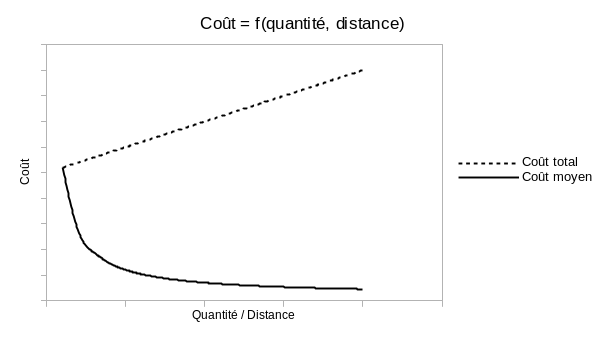
\includegraphics[width=12cm]{f2_1.png}}
\caption{\label{f2_1} Relation entre la quantit\'e/distance et le co\^ut}
\end{figure}


Toutefois, les coûts totaux sur les arcs ne sont pas toujours linéaires par
rapport à la quantité transportée. C'est ainsi que les coûts de manutention ne
sont pas linéaires par rapport à la quantité de marchandises à charger ou
décharger.



Dès le moment où il faut tenir compte des phénomènes de congestion, il  faut
introduire le flux (quantité totale transportée sur un arc déterminé) comme
variable explicative du coût. Le coût total de transport évolue alors de manière
exponentielle par rapport à ce flux, comme illustré dans la figure \ref{f2_2}

\begin{figure}[htbp]
\centerline{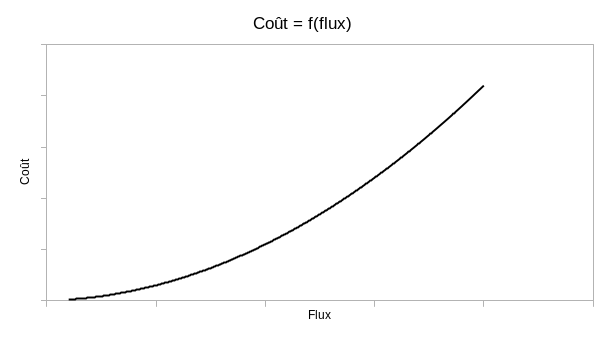
\includegraphics[width=12cm]{f2_2.png}}
\caption{\label{f2_2} Relation Co\^ut-Flux}
\end{figure}


Reste maintenant à considérer le coût total sur le système de transport. Bien
qu'il existe différentes méthodes d'affectation du flux sur un réseau, elles ont
toutes en commun le fait de minimiser une fonction objectif. Ces fonctions
objectif peuvent également prendre différentes formes. C'est ainsi qu'en se
plaçant du point de vue de la collectivité, il s'agit de minimiser le coût total
de transport sur le système. Par contre, il faudra minimiser le coût moyen des
voyages s'il s'agit du point de vue de l'usager.

D'une manière générale, lorsque les fonctions de coût de transport sont
linéaires par rapport aux quantités, et que la congestion ne doit pas être
modélisée, en sorte qu'il est toujours possible d'affecter les transports en
choisissant la solution (choix d'un mode, d'un moyen ou d'une route) de coût
minimum par la mise en oeuvre d'un bon algorithme de recherche de chemin sur un
graphe, il n'y a pas à proprement parler de fonction objectif dans la mesure où
il y a discontinuité entre les différentes solutions possibles. Cependant, si
les coûts des différentes combinaisons convexes des solutions de répartition des
quantités sont distingués, la fonction de coût obtenue serait une fonction
linéaire (non strictement convexe), car toutes les fonctions de coûts sur les
différents segments sont linéaires par rapport aux quantités transportées sur ce
segment.

Par contre, lorsque des fonctions de coût non linéaires (convexes)
sont utilisées sur les arcs, ce qui doit être le cas pour les
modèles qui tiennent compte du niveau de congestion sur le réseau,
les solutions ne seront en général pas du type ``tout ou rien``,
mais il y aura une répartition des quantités entre les différents
modes, moyens et routes disponibles. L'ensemble de ces solutions
potentielles forme alors une fonction de coût total continue
convexe résultant de la sommation des différentes fonctions
convexes.



Il y a plusieurs concepts de coûts à prendre en considération et c'est la raison
pour laquelle, tout au long de ce texte, il sera bien précisé ce à quoi les
coûts utilisés font référence.



\subsection{Le comportement des acteurs sur un syst\`eme de transport}

Les étapes de génération et de distribution du modèle classique à
quatre étages sont des approches plutôt agrégées de la décision de
transport. Ce n'est qu'au moment où il faut réellement se pencher
sur le choix d'un mode de transport et sur le choix d'une route à
emprunter sur un réseau que les comportements des acteurs dans le
système de transport sont analysés plus en profondeur, sous un
angle plus pointu.

Classiquement, les acteurs considérés sont les producteurs de biens (qui jouent
le rôle d'expéditeur), les consommateurs et les transporteurs. Les producteurs
et les consommateurs ne sont pas localisés au même endroit. L'analyse des
mécanismes qui régissent les liens entre ces différents acteurs est la raison
même de l'existence de l'économie des transports et de tous les outils
informatiques, tels que NODUS, qui ont été développés ces dernières années.


Les expéditeurs sont l'ensemble des agents économiques qui prennent la décision
d'affecter et de distribuer un certain flux de marchandises entre une origine et
un certain nombre de destinations. Les transporteurs représentent en réalité un
ensemble de différentes entités impliquées dans la décision de transport. On y
trouve par exemple les département ``expéditions``, ``distribution`` ou
``réception`` des firmes. La décision de transport peut être quelque chose de
complexe, mais comme le dit si bien Roberts \footnote{Roberts, P.O., 1976,
``Forecasting Freight Flows Using a Disaggregated Freight Demand Model``, CTS
Report 76-1, Center for Transportation Studies, MIT.},``la seule motivation qui
pousse au déplacement de la marchandise est la raison économique``. Dès lors, la
décision du transporteur dépend du comportement de l'offre et de la demande et
des prix (de la marchan\-dise) sur le marché.

Lorsque l'expéditeur prend sa décision de transport, il choisit un
transporteur pour effectuer le transport. En économie des
transports, le transporteur est toujours perçu comme un agent
économique qui produit du transport en essayant de maximiser son
profit.

La relation entre les expéditeurs et les transporteurs est
assimilée à celle qui peut exister entre un consommateur et un
producteur de services. Par sa décision d'attribuer un chargement à
un transporteur, l'expéditeur crée une demande pour l'output
produit par ce transporteur. De son côté, le transporteur va
demander un certain prix pour effectuer le transport et crée de ce
fait un certain niveau de service.

Si on ajoute à cela le rôle joué par l'état, on peut représenter les relations
existantes entre les différents acteurs de la manière présentée dans la figure
\ref{f2_3}:

\begin{figure}[htbp]
\centerline{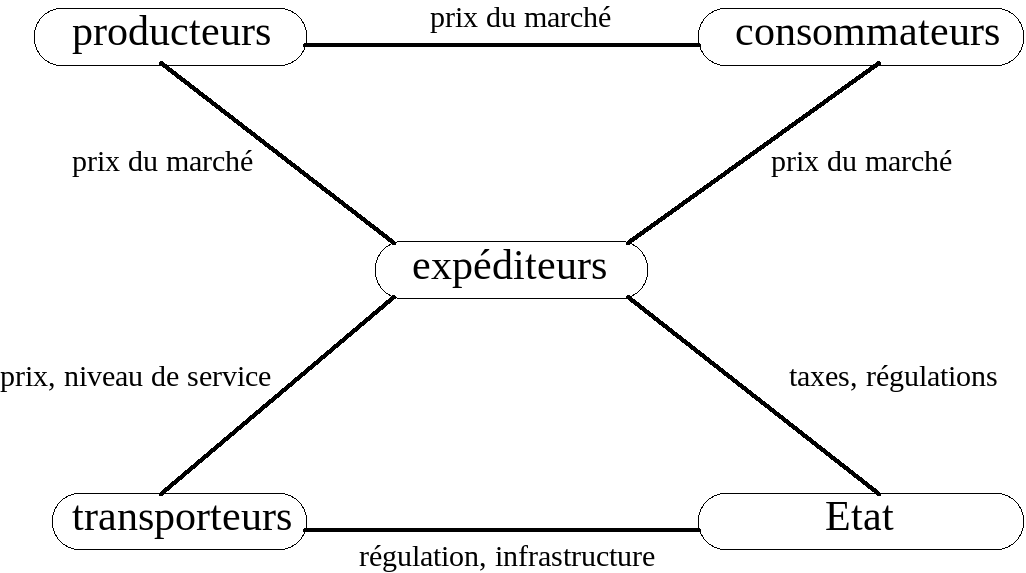
\includegraphics[width=10cm]{f2_3.png}}
\caption{\label{f2_3} Les acteurs d'un syst\`eme de transport}
\end{figure}


Il reste néanmoins évident que toutes ces interactions ne peuvent
exister que dans la mesure où il existe une demande pour le
transport. Cette dernière est fonction de différents facteurs
explicatifs parmi lesquels:

\begin{itemize}

\item Le prix du service de transport: comme la demande de n'importe quel
bien, la demande de transport est en principe une relation
décroissante du prix du transport.

\item Le prix des autres modes de transport: alors que certaines catégories
de marchandises sont transportées (presque) uniquement par un seul
mode de transport, certaines catégories peuvent voyager par des
modes différents. Une variation du prix sur un mode de transport
peut de ce fait influencer la demande pour un autre mode.

\item Le prix des biens complémentaires: on peut considérer le transport comme
faisant partie d'un processus de production. Un exemple classique
est celui de la production d'énergie électrique par des centrales
thermiques qui doivent faire venir le combustible (charbon, fuel)
par péniche ou par camion. Il est évident que la demande de
transport pour le combustible est directement fonction du niveau de
production d'énergie.

\item La durée: le transport est un bien extrêmement particulier dans la mesure
où son utilisateur est ``impliqué`` dans la production du service de transport
par le temps que la marchandise passe à se déplacer. La durée du transport joue
un rôle capital pour expliquer la demande de transport et le choix modal. La
demande de transport est en relation inverse avec la durée nécessaire au
transport. L'élasticité-temps est donc négative. La demande de transport est
également sensible à la vitesse, mais cette dernière apparaît davantage comme un
élément déterminant la durée du transport que comme un facteur explicatif
supplémentaire.

\item La liberté de disposition: les expéditeurs sont très sensibles à ce
facteur, qui explique en partie le succès du transport routier.

\item La capacité: l'adéquation entre les caractéristiques des marchandises à
transporter (volume, poids) et celles du mode de transport détermine souvent le
choix du mode.

\item La sécurité et le respect des délais. les transports de marchandises
sont sensibles aux risques encourus (bien que la perception de ce
risque est souvent subjective) et au respect des délais
d'exécution.

\end{itemize}



\section{Techniques de g\'en\'eration et de distribution}

Cette section présente quelques techniques de
base qui concernent la génération et la distribution\footnote{Le lecteur
intéressé par une présentation plus approfondie de ces techniques lira avec
intérêt le livre de J. de D. Ortuzar et L. G. Willumsen, ``Modelling
Transport``, Wiley, 2011.}. Pour rappel, NODUS ne contient pas de modules de
génération et de distribution: les matrices O-D doivent donc toujours être
fournies, et les quelques paragraphes qui suivent doivent être considérés comme
une petite présentation théorique, utile lorsque des matrices O-D ne sont pas
disponibles ou lorsqu'elles sont partielles ou anciennes. La génération permet
en effet d'estimer les flux totaux en provenance et à destination des
différentes zones du réseau tandis que la distribution permet de créer une
matrice O-D à partir de ces flux totaux.

Encore une fois, les pages qui suivent n'ont aucunement la prétention de
présenter un état complet de l'art en la matière, l'objectif étant simplement
ici d'aider le lecteur non familiarisé avec les techniques de base de la
modélisation classique.

\subsection{G\'en\'eration}

L'étape de génération essaye de déterminer l'attraction et l'émission globale de
chaque zone de l'aire géographique étudiée. A ce stade, les liens qui peuvent
exister entre une origine et une destination particulière ne sont pas encore
pris en considération. Les mouvements qui vont et viennent d'un noeud déterminé
sont estimés en classant les flux par catégorie (objectif, période, type de
marchandise, ...) et en déterminant les facteurs qui influencent ces flux. Dans
le cas du transport de marchandises, les critères suivants sont généralement
pris en considé\-ration :

\begin{itemize}
\item la nature des marchandises,
\item la population,
\item le niveau de revenus,
\item nombre d'employés dans les entreprises,
\item le nombre de transactions réalisées,
\item la zone d'influence des firmes,
\item etc.
\end{itemize}

Ces données sont ensuite essentiellement exploitées par:

\begin{itemize}
\item des analyses de régression,
\item des techniques de classification croisées,
\item des techniques de prévision sur les variables utilisées,
\item des techniques de test de stabilité des résultats obtenus.
\end{itemize}

\subsection{Distribution}

L'étape suivante consiste logiquement à distribuer les flux totaux
entre les différents pôles mis en évidence dans l'étape de
génération. En d'autres termes, il s'agit maintenant d'estimer une
matrice O-D.

La littérature présente plusieurs méthodes dont les plus classiques sont les
méthodes du taux de croissance et les méthodes synthétiques.

\subsubsection{Les méthodes du taux de croissance.}

Ces méthodes se basent sur l'existence préalable d'une première
matrice O-D (t). L'utilisation d'un taux de croissance attendu
permet alors d'estimer une nouvelle matrice.

La méthode de base est utilisée seulement d'un taux de croissance
général est disponible  $\tau$. On applique alors $T_{ij} = \tau
t_{ij}$ pour chaque paire ij.

Si un taux de croissance spécifique est disponible pour chaque
origine ou chaque destination $\tau_i$ ou $\tau_j$, on parle de la
méthode du taux de croissance à une seule contrainte.

Dans ce cas, $T_{ij} = \tau_it_{ij}$ pour un taux de croissance
"origine" et $T_{ij} = \tau _jt_{ij}$ pour un taux de croissance
"destination".

Par exemple (voir tableau \ref{tab2_1}), avec une information prévisionnelle de
flux sur les origines (cibles).

\begin{table}[htbp]
\begin{center}
\begin{tabular}{rrrrrrr}
\hline
i$\backslash$j & 1 & 2 & 3 & 4 & $\sum\limits_{i}$ & Cibles $O_i$\\
\hline
1 & 5 & 50 & 100 & 200 & 355 & 400\\ 2 & 50 & 5 & 100 & 300 & 455 & 460\\

3 & 50 & 100 & 5 & 100 & 255 & 400\\ 4 & 100 & 200 & 250 & 20 & 570 & 702\\
$\sum\limits_{i}$ & 205 & 355 & 455 & 620 & 1635 & 1962\\
\hline
\end{tabular}
\caption{\label{tab2_1} Pr\'evision aux origines et destinations}
\end{center}
\end{table}


Le problème peut facilement être résolu en multipliant chaque ligne par le ratio
$O_i/\sum\limits_jt_{ij}$ , qui représente un taux de croissance (voir tableau
\ref{tab2_2}).

\begin{table}[htbp]
\begin{center}
\begin{tabular}{rrrrrrr}
\hline
i$\backslash$j & 1 & 2 & 3 & 4 & $\sum\limits_{i}$ & Cibles $O_i$\\
\hline
1 & 5.6 & 56.3 & 112.7 & 225.4 & 400 & 400\\

2 & 50.5 & 5.1 & 101.1 & 303.3 & 460 & 460\\

3 & 78.4 & 156.9 & 7.8 & 156.9 & 400 & 400\\

4 & 123.2 & 246.3 & 307.9 & 24.6 & 702 & 702\\

$\sum\limits_{i}$ & 257.7 & 464.3 & 529.5 & 701.2 & 1962 & 1962\\
\hline
\end{tabular}
\caption{\label{tab2_2} Application du ratio de croissance}
\end{center}
\end{table}



La méthode du taux de croissance à double contrainte est appliquée lorsque des
estimations sur le nombre futur de mouvements aux origines et aux destinations
sont disponibles. On dispose dans ce cas, pour chaque noeud, d'un facteur de
croissance d'attraction $\tau_i$ et de génération $\Gamma_j$. L'utilisation d'un
facteur moyen $F_{ij}=0.5(\tau_i+\Gamma_j)$ n'est qu'un compromis très
approximatif. Pour résoudre ce problème, on a recours à des processus itératifs,
dont le plus connu est celui de Furness
\footnote{ Furness K. P., 1965, ``Time Function Iteration``,
Traffic Engineering and Control, 7(7), 458-60} qui introduit la
notion de ``facteurs de balancement`` $A_i$ et $B_j$.

\begin{center}
$$T_{ij} = t_{ij}\tau_i\Gamma_jA_iB_j$$
ou encore
$$T_{ij} = t_{ij}a_ib_j ~avec~ a_i = \tau_iA_i ~et~ b_j = \Gamma_jB_j$$
\end{center}

Le processus itératif est le suivant:


\begin{itemize}
\item Initialiser tous les $b_j$ à 0 et résoudre pour $a_i$ (satisfaire la
contrainte de génération).
\item Calculer les $b_j$ en utilisant les $a_i$ obtenus précédemment
(satisfaire la contrainte d'attraction).
\item Recalculer les $a_i$ avec les $b_j$ obtenus. Répéter les étapes
précédentes jusqu'à obtention de paramètres stables.%
\end{itemize}


Les méthodes basées sur le taux de croissance sont simples car
elles se basent sur la pré-existence de matrices O-D observées et
de taux de croissance estimés. L'utilisation de matrices O-D
pré-existantes constitue évidemment leur point faible. En effet, il
n'est dès lors possible que de réaliser des prévisions à court
terme sur des réseaux qui restent fort stables.



\paragraph{Les méthodes synthétiques.}


Différentes méthodes ont été mises au point pour réaliser des prévisions sur des
réseaux qui sont amenés à connaître, par exemple, de grandes variations de flux.
La plus connue de ces méthodes est le modèle de gravité, dont la formulation
générale est:


$$T_{ij} = \alpha O_iD_jf(c_{ij})$$


où $O_i$ et $D_j$ représentent les émissions et attractions totales, $\alpha$
est un facteur de proportionalité et $f(c_{ij})$ est une fonction de coût de
transport généralisé connue sous le nom de ``fonction de dissuasion
\footnote{Par exemple:
\begin{itemize}
\item exponentielle $f(c_{ij}) = exp(-\beta c_{ij})$
\item puissance $f(c_{ij}) = c_{ij}^n$
\item combinée $f(c_{ij}) = c_{ij}^nexp(-\beta c_{ij})$
\end{itemize} }.
`` (deterence function).

Le modèle de gravité repose sur le principe que la probabilité de réaliser un
voyage entre deux noeuds ``proches`` est plus grande que celle d'effectuer un
voyage entre deux noeuds ``éloignés``. Le concept de distance doit ici être
consi\-déré dans son sens le plus large. En effet, si la distance physique peut
être utilisée comme facteur de proportionalité, deux noeuds peuvent également
être consi\-dérés comme ``proches`` s'ils ont le même type d'activité économique
ou des activités économiques complémentaires. C'est ainsi qu'il y a plus de
trafic entre deux régions industrielles qu'entre deux régions agricoles.

Lorsqu'une contrainte (simple ou double) est introduite, on utilise
le processus de Furness en utilisant les facteurs de balancement
$A_i$ et $B_j$ en lieu et place du facteur $\alpha$:

$$T_{ij}=A_iO_iB_jD_jf(c_{ij})$$

Dans le cas du modèle à simple contrainte, $A_i$ ou $B_j$ est égal
à l'unité. En effet, dans le cas contraire, l'interdépendance des
facteurs de balancement exige un processus itératif, comme celui
expliqué plus haut.

Exemple avec fonction de détérence exponentielle %
\footnote{Divers chercheurs ont essayéde proposer des estimations pour le
paramètre $\beta$. Voir par exemple Blauwens G., 1975, ``Interpreting
Coefficients in Gravity Model``, werknota 32, UFSIA-SESO, Anvers} $(\beta
=.10)$ (voir tableaux \ref{tab2_3} à \ref{tab2_5}).

\begin{table}[htbp]
\begin{center}
\begin{tabular}{rrrrrr}
\hline
%\multicolumn{5}{c}{Coût en minutes} & Cibles (flux)\\
 & & & & & Cibles (flux)\\
i$\backslash$j & 1 & 2 & 3 & 4 & $O_i$\\
\hline
1 & 3 & 11 & 18 & 22 & 400\\

2 & 12 & 3 & 13 & 19 & 460\\

3 & 15.5 & 13 & 5 & 7 & 400\\

4 & 15.5 & 13 & 5 & 7 & 400\\

$D_j$ & 260 & 400 & 500 & 802 & 1962\\
\hline
\end{tabular}
\caption{\label{tab2_3} Matrice des co\^uts (en minutes)}
\end{center}
\end{table}



\begin{table}[htbp]
\begin{center}
\begin{tabular}{rrrrrr}
\hline
%\multicolumn{5}{c}{$exp(-\beta cost)$} & Cibles (flux)\\
& & & & & Cibles (flux)\\
i$\backslash$j & 1 & 2 & 3 & 4 & $O_i$\\
\hline
1 & 0.74 & 0.33 & 0.17 & 0.11 & 400\\

2 & 0.30 & 0.74 & 0.27 & 0.15& 460\\

3 & 0.14 & 0.27 & 0.61 & 0.50 & 400\\

4 & 0.09 & 0.17 & 0.45 & 0.61 & 702\\

$D_j$ & 260 & 400 & 500 & 802 & 1962\\
\hline
\end{tabular}
\caption{\label{tab2_4} R\'esultats de la fonction de d\'et\'erence $exp(-\beta cost)$}
\end{center}
\end{table}


\begin{table}[htbp]
\begin{center}
\begin{tabular}{rrrrrrr}
\hline
i$\backslash$j & 1 & 2 & 3 & 4 & $O_i$ & $a_i$\\
\hline
1 & 162 & 98.5 & 65.5 & 74 & 400 & 405.2\\

2 & 162 & 98.5 & 65.5 & 74 & 400 & 405.2\\

3 & 18.2 & 47.2 & 140.6 & 194 & 400 & 237.1\\

4 & 23.4 & 55.4 & 192.2 & 431 & 702 & 439.4\\

%$D_j$ & 265.1 & 405.6 & 499.1 & 792.2 & \multicolumn{2}{c}{$1962 / 1959.9$}\\
$D_j$ & 265.1 & 405.6 & 499.1 & 792.2 & & $1962 / 1959.9$\\


$b_j$ & 1.5 & 1.7 & 2.0 & 2.6 & &\\
\hline
\end{tabular}
\caption{\label{tab2_5} Matrice de gravit\'e}
\end{center}
\end{table}



\section{Techniques de choix modal}

La notion de réseau virtuel, telle qu'elle est mise en oeuvre dans le logiciel
NODUS, combine les étapes de choix modal et de génération du modèle classique à
quatre étages. Néanmoins, il est utile ici de présenter les techniques
alternatives afin de mieux comprendre l'apport du réseau virtuel en terme de
facilité de modélisation.

L'analyse des facteurs qui déterminent le choix modal a toujours
retenu l'atten\-tion pour l'étude de la concurrence entre les modes
de transport. Pour ce faire, une large palette de modèles a été
mise au point. D'après Wilson
\footnote{Wilson A. G., 1981, ``A Disaggregate Model of the Demand
for Intercity Freight Transportation``, Econometrica, 49,
981-1006.}, les modèles de demande peuvent être classés en deux
catégories: les modèles agrégés et les modèles désagrégés. Ceux-ci
se distinguent surtout par le niveau d'agrégation des données qui
sont utilisées.

Selon le niveau d'agrégation des données, le tableau \ref{tab2_6} peut être
établi.

\begin{table}
\begin{center}
\begin{tabular}{ll}
\hline
Niveau d'agrégation & Modèles\\
\hline
Agrégé& Modèles de demande dérivée\\

& Modèles probabilistes\\

Désagrégé& Modèles probabilistes\\

& Théorie des inventaires\\
\hline
\end{tabular}
\caption{\label{tab2_6} Types de mod\`eles en fonction du niveau d'aggr\'egation}
\end{center}
\end{table}



\subsection{Mod\`eles agr\'eg\'es}


Les modèles agrégés considèrent que les producteurs maximisent leur
profit et que le transport doit être inclus dans leur processus de
production. La fonction de demande de transport est donc basée sur
la fonction de coût estimée de la firme.

L'approche agrégée implique l'utilisation de séries temporelles
et/ou croisées pour estimer des relations structurelles qui
décrivent le comportement d'un ou de plusieurs acteurs du système
de transport. L'objectif de ce type d'approche est habituellement
l'estimation de fonctions de coût ou de production générales
applicables à une firme particulière ou à une industrie toute
entière. D'une manière générale, cette approche ignore le détail
d'un réseau de transport: elle ne convient donc pas pour analyser
les flux sur un réseau complexe. Leur présentation ne répond dès
lors qu'au seul souci d'exhaustivité.

\subsubsection{Mod\`eles de demande d\'eriv\'ee}


Les travaux de Sloss\footnote{Sloss J., 1971, ``The Demand for Intercity Motor
Freight Transport: a Macroeconomic Analysis``, The Journal of Business,
janvier.}, de Oum, \footnote{ Oum T. H., 1977, ``Derived Demand for Freight
Transportation and Inter-Modal Substitutibilities in Canada``, Transportation
Research Forum Conference Proceedings XVIII(1), 56-57.} et de Friedlander et
 Spady \footnote{ Friedlander A. F. et Spady R. H., 1981, ``Freight
Transport Regulation: Equity, Efficiency and Competition in the
Rail and Trucking Industries``, MIT Press, Cambridge, MA.} relèvent
de ce type d'approche. Les fonctions de coût y sont spécifiées
comme dans la théorie néo-classique de la production, où
l'expéditeur est censé minimiser son coût de transport sous
différentes contraintes technologiques.


L'approche adoptée est la fonction translogarithmique, qui n'impose
pas de restrictions aux élasticités prix et de substitution. Ces
fonctions appartiennent à la famille des fonctions dites flexibles
et pouvant être utilisées afin d'obtenir une approximation du
second ordre de la série de Taylor.


Oum utilise des données agrégées en série chronologique portant sur
les flux de marchandises entre certaines villes canadiennes, tandis
que des données en coupe instantanée, plus désagrégées, sont
utilisées par Friedlander et Spady.


Les modèles de demande dérivée considèrent le transport comme un
input nécessaire d'un processus de production. De ce fait, la
demande de transport est dérivée de l'output produit. De façon
analytique, les fonctions de demande d'inputs de transport
utilisées par Oum et par Friedlander et Spady sont obtenues dans un
contexte de concurrence parfaite à l'aide du lemme de Sheppard
\footnote{ Sheppard E. et Curry L., 1982, ``Spatial Price
Equilibria``, Geographical Analysis 14, 279-304.}. L'utilisation
des fonctions de coût, et non des fonctions de production, se
justifie par la relation de dualité liant ces deux expressions.


La base même de ce type d'approche est donc une seule et unique fonction, de
type translogarithmique, qui s'adapte bien à des données agrégées. Il semble
évident qu'il n'est pas possible de l'utiliser directement sur un réseau,
composé d'un grand nombre d'arcs et de noeuds qui sont autant d'éléments
auxquels il faut affecter un coût (ou une estimation de coût). On ne peut
néanmoins pas rejeter l'idée que l'expéditeur essaye de minimiser ses coûts.


\subsubsection{Mod\`eles probabilistes}

Cette approche a été utilisée par plusieurs auteurs, sous la forme
de modèles logit.

Le modèle logit (multinomial) se présente de la manière suivante:

$$P_n(i)=\frac{e^{V_{in}}}{\sum\limits_{j\in C_n}e^{V_{jn}}}$$
avec:

$$0 \leq P_n(i) \leq 1$$

$$\sum \limits_{i \in <c_n}P_n(i) = 1$$


où:

\begin{itemize}
\item $P_n(i)$: probabilité que l'alternative i soit choisie parmi les n
possibilités
\item $V_{in}$ et $V_{jn}$: composantes systématiques (représentatives)
de la fonction d'utilité de i et de j
\item $C_n$: choix possibles
\end{itemize}


Le modèle multinomial se caractérise par le fait que le décideur a
le choix entre plus de deux alternatives parmi un ensemble $C_n$
d'alternatives:

$$U_{in}=V_{in}+\epsilon _{in}$$

où $\epsilon _{in}$ représente le bruit aléatoire.


Etant donné que les modèles probabilistes sont également repris dans la section
``modèles désagrégés``, nous ne pousserons pas plus loin notre exploration,
d'au\-tant plus que l'approche agrégée se prête assez mal à des études basées
sur des réseaux de transport nécessitant un niveau de détail important. Par
ailleurs, la topologie du réseau joue également un grand rôle dans le choix
modal et cette dynamique est souvent, si pas toujours, ignorée à un niveau élevé
d'agrégation.


\subsection{Mod\`eles d\'esagr\'eg\'es}

\subsubsection{Mod\`eles probabilistes}


L'approche probabiliste a également été utilisée à un niveau
désagrégé.
 Daughety et Inaba \footnote{Daughety A. F. et Inaba F.S., 1978,
``Estimation of Service-Differentiated Transport Demand
Functions``, Transportation Research Record, 668, 23-30.}, par
l'introduction d'une composante aléatoire au niveau du profit, ont
formulé les modèles logit, souvent utilisés
\footnote{Par exemple:
\begin{itemize}
\item Daughety A. F., 1979, ``Freight Demand Transport Revisited: A
Microeconomic View of Multi-Modal Multi-Characteristic Service
Uncertainty and Demand for Freight Transport``, Transportation
Research, 13, 281-288.
\item Daughety A. F. et Inaba F.S., 1981, ``An Analysis of Regulatory Change
in the Transportation Industry``, Rev. of Econ. and Stat., 53,
246-255.
\item Levin R. C., 1981, ``Railroad Rates, Profitability and Welfare under
Deregulation``, Bell J. of Econ., 12, 1-26.
\end{itemize}} . Ce type de modèle suppose que l'expéditeur peut être représenté
par un certain vecteur caractéristique S qui reflète indirectement ses goûts.
Cet expéditeur a le choix entre plusieurs modes de transport qui peuvent être
représentés par des vecteurs d'attributs X. La fonction d'utilité associée à un
mode peut être représentée de la façon suivante:

$$\cup =V(S,X)+\epsilon (S,X)$$

où $V$ est une fonction non stochastique reflétant les goûts représentatifs de
la population alors que le caractère particulier d'un expéditeur donné se
caractérise par la fonction aléatoire .

Dans le cas où seulement deux modes sont utilisés, si $X^1$ et $X^2$ sont
respec\-tivement les caractéristiques des modes 1 et 2, le mode 1 sera choisi si:

$$V(X^1,,S)+\epsilon (X^1,S) > V(X^2,S) + \epsilon (X^2,S)$$


Le comportement d'aversion au risque a été analysé plus en profondeur par Wilson
\footnote{ Wilson A. G., 1981, ``A Disaggregate Model of the Demand for
Intercity Freight Transportation``, Econometrica, 49, 981-1006.}. Pour cet
auteur, cette aversion n'est pas la même pour tous les modes de transport.
L'hypothèse d'indépendance de l'erreur stochastique, nécessaire pour dériver un
modèle logit, peut ne pas être réaliste. Une hypothèse plus plausible de
distribution des erreurs voudrait que celles-ci soient indépendam\-ment
distribuées et suivent une distribution normale. Le modèle qui en résulte est le
modèle probit.


\subsubsection{Mod\`eles d\'eriv\'es de la th\'eorie des inventaires}


L'approche de la valeur d'inventaire cherche à optimiser le comportement de
recherche de profit de l'expéditeur. Baumol et Vinod \footnote{ Baumol W.J. et
Vinod H.D.,1970, ``An Inventory Theoretic Model of Freight Transportation
Choice``, Management Science, 16, 413-21} ont été les précurseurs dans cette
voie. Ils ont étésuivis par Das \footnote{ Das C. (1972), ``Choice of Transport
Service: An Inventory Theoretic Approach``, The Logistics and Transportation
Review, 10, 181-87}, et Constable et Whybark \footnote{ Constable G.K. et
Whybark D.C.,1978, ``The Interaction of Transportation and Inventory
Decisions``, Decision Science, 3, 688-99}. Bien que relativement ancienne, cette
approche n'est utilisée dans des modèles empiriques que depuis une bonne
quinzaine d'années, entre autres par Allen \footnote{ Allen W. B., 1977, ``The
Demand for Freight Transportation: A Micro Approach``, Transportation Research
11, 9-14.}, Chiang et Roberts
\footnote{Chiang Y.S. et Roberts P.O.,1980, ``A Note on Transit
Time and Reliability for Regular-Route Trucking``, Transportation Research, 14B,
59-65.}, et McFadden et Winston \footnote{McFadden D. et Winston C., 1981,
``Joint Estimation of Discrete and Continuous Choices in Freight
Transportation``, Meeting of the Econometric Society.}.

Le modèle se base sur une fonction de profit qui tient compte de la
valeur d'inventaire de la marchandise au début et à la fin de
l'envoi. Il s'agit donc ici de déterminer la quantité et la
fréquence optimale des envois, afin de maximiser le profit des
entreprises. L'expression de base de cette approche est:

$$CT = C_s + C_t + C_i$$

où:

\begin{itemize}
\item $C_s$ : coùts directs annuels de transport
\item $C_t$ : couts financiers annuels dus à la détention de la marchandise
durant le transport
\item $C_i$ : coûts annuels d'ordre administratif + coûts liés aux stocks de
sécurité\end{itemize}

La mise en place d'un tel modèle nécessite évidemment une grande
quantité de données, dans la mesure où il faut exprimer les coûts
de transport en fonction de la taille du chargement, des coûts de
détention de la marchandise, de la demande du bien, etc...

L'approche est cependant fort intéressante car elle tient compte explicitement
de la marchandise dans le processus de décision. De plus, la nature désagrégée
de cette technique s'adapte bien aux méthodes de réseau, car les différents
éléments de coût qui composent ce modèle peuvent être affectés à des arcs ou à
des noeuds d'un réseau. La recherche d'un chemin, qui correspond finalement à la
décision de transport, peut alors être réalisée au travers de la mise en oeuvre
d'un algorithme de la théorie des graphes, sans faire appel à des notions de
probabilités de choix.

Bien que, à l'origine, ce type de modèle n'ait pas été dévveloppé dans une
optique de réseau, il s'agit de la technique qui est la plus facilement
transposable. C'est donc sur cette base théorique que s'appuiera le choix modal
effectué lors de la mise en oeuvre du réseau virtuel.

\subsection{Conclusions sur les techniques de choix modal}

Qu'elles soient agrégées ou non, les techniques de choix modal ne répondent
qu'incomplètement à la dynamique des réseaux.

Les techniques agrégées ne conviennent pas bien à une utilisation sur un réseau.
Il en va de même de l'approche désagrégée probabiliste. Dans les deux cas en
effet, il est difficile de prendre en considération le détail des réseaux.

L'approche dérivée de la théorie des inventaires servira donc de source
d'inspi\-ra\-tion lors du développement des fonctions de coût spécifiques qui
seront utilisées lors de la mise en oeuvre du réseau virtuel. De plus, alors que
l'approche originelle s'attache uniquement à maximiser le profit des
expéditeurs, les modèles gérés par NODUS prendront en considération les coûts
supportés par les transpor\-teurs par le biais de la recherche des itinéraires les
moins chers.

Il reste néanmoins évident que les critères qui mènent à la décision du choix de
mode de transport ne sont pas uniquement d'ordre purement monétaire. C'est ainsi
qu'il faut prendre en considération des éléments aussi divers que la durée du
voyage, la facilité de chargement ou la catégorie de marchandises qui est
transportée. Tous ces critères tendent à donner un certain niveau de qualité (au
sens large) d'un mode de transport.


\section{Techniques d'affectation}

Les méthodes d'affectation, qui visent à affecter les matrices O-D sur le réseau
en minimisant les coûts (généralisés), peuvent se classer en quatre grandes
catégories, selon qu'elles tiennent compte ou non des contraintes de capacité
liées au réseau et de l'aspect linéaire ou non de la fonction objectif (voir
tableau \ref{tab2_7}). Cette fonction objectif peut par ailleurs prendre
différentes formes selon le point de vue adopté dans un modèle. Lorsque l'on
s'attache à optimiser l'ensemble d'un système de transport, on choisira de
minimiser les coûts totaux, alors que pour un modèle d'équilibre ``usagers``, on
minimisera les coûts moyens.


\begin{table}[htbp]
\begin{center}
\begin{tabular}{llll}
\hline
& & Comp. non stochastique & Comp. stochastique \\
\hline
Cont. de capacité& Non & Tout ou rien & Multi-flots\\
& Oui & Equilibre classique & Equilibre mutli-flots\\
\hline
\end{tabular}
\caption{\label{tab2_7} Techniques d'affectation}
\end{center}
\end{table}


Dans les modèles d'équilibre et multi-flots, il peut y avoir plusieurs chemins utilisés entre
les mêmes origine et destination, alors que le modèle ``tout ou rien`` recherche un seul 
chemin par paire O-D. Seul le modèle d'équilibre multi-flots n'est pas impléménté dans Nodus.

Par rapport au modèle ``tout ou rien``, le modèle d'équilibre classique tient
compte du trafic existant pour rechercher un chemin dans le réseau au travers de
fonctions de coût du type ``volume-délai``, ce qui revient à prendre en compte
la capacité de manière implicite.

Indépendamment de ce qui est publié dans le tableau précédent, les techniques
d'affectation peuvent tenir compte ou non de l'aspect stochastique du
compor\-te\-ment des usagers.


Les méthodes stochastiques ont surtout été développées pour le
transport de personnes \footnote{Les modèles les plus connus sont
ceux de:
\begin{itemize}
\item Dial R.B., 1969, ``A Probabilistic Multipath Traffic Assignment
Model wich Obviates Path Enumeration``, Transportation Research, 5,
83-112.
\item Gunarsson S.O., 1972, ``An Algorithm for Multipath Traffic Assignment``,
PTRC Seminar Proceedings, Urban Traffic Model Research, 8-12 May.
\item Randle J., 1979, ``A Convergent Probabilistic Road Assignment
Model``, Trafic Eng. and Control, 20, 519-521. Ce modèle est plus
connu sous le nom de G.M.T.U. (Greater ManchesterTransportation
Unit).
\end{itemize}}. En effet, la perception que différents voyageurs ont de leur
environ\-ne\-ment n'est pas la même. Un conducteur peut par exemple préférer
l'autoroute pour se rendre d'un point à un autre, alors que son voisin préfèrera
une route nationale. Cette préférence se traduit par la notion d'utilité. Pour
pouvoir mettre en oeuvre de tels modèles, les utilisateurs sont supposés avoir
une perception de l'utilité de chaque itinéraire possible. On fait alors souvent
l'hypothèse qu'ils tendent à choisir le chemin qui maximise leur utilité. La
représentation de tels comportements fait appel à des modèles probabilistes plus
ou moins complexes selon que l'utilisateur a le choix entre deux (logit,
probit,...) ou plusieurs (logit multinomial, Dial, ...) itinéraires.


Bien sûr, le transport de marchandises peut aussi être affecté par ce genre de
considérations, surtout s'il s'agit de transports en milieu urbain lors desquels
des problèmes de congestion peuvent être rencontrés, mais l' attention se
portera ici plutôt sur les méthodes non stochastiques car les problèmes de
transport multi-modaux ne se conçoivent que sur des distances relativement
longues et sur des réseaux nationaux ou internationaux.


Lorsque l'on s'attache à des problèmes liés aux réseaux,
l'affectation passe également par la mise en oeuvre d'algorithmes
de recherche de chemins les plus courts (ou les moins coûteux) tel que l'algorithme 
de Dijkstra mis en oeuvre dans NODUS. Le choixd'un algorithme de recherche de 
chemin n'influence pas la solution du problème économique posé par 
l'affectation: seuls les temps de calcul sur un ordinateur s'en trouvent affectés.


\subsection{Le ``tout ou rien``}

Les modèles qui mettent en oeuvre une méthode d'affectation de type ``tout ou
rien`` font l'hypothèse que le réseau n'est pas limité par des contraintes de
capacité. On affecte donc l'ensemble des quantités à transporter reprises dans
la matrice O-D sans aucune contrainte. Malgré cette limitation, les méthodes du
type ``tout ou rien`` sont encore largement utilisées à certaines étapes d'une
étude. Elles se justifient sur de grands réseaux faiblement chargés ou pour
visualiser les flux dans des situations non contraignantes.


Dans des applications de type macroscopique, il importe souvent peu de savoir si
un carrefour est encombré. Par contre, il est important de savoir qu'il faut
tenir compte d'un certain temps pour traverser telle ou telle ville. Ce genre de
considération se matérialise d'ailleurs au travers de la topologie du réseau qui
est utilisé: le détail des zones urbaines (rues, carrefours,...) n'est pas
digitalisé lorsque l'on travaille sur de gros réseaux, tels que le réseau
européen. La conges\-tion peut alors être prise en compte par un coût
supplémentaire (congestion, passage aux frontières, ...) à imputer aux noeuds du
réseau, et une méthode ``tout ou rien`` peut alors se justifier. NODUS permet
évidemment de réaliser des affectations de ce type.



\subsection{M\'ethodes d'\'equilibre}


Il paraît évident qu'à un moment ou un autre, des phénomènes de
congestion apparaissent. Il s'agit donc d'introduire, lors de la
phase d'affectation, une méthode qui puisse résoudre les
contraintes liées à la capacité du réseau. L'une des solutions les
plus utilisées pour résoudre les problèmes de congestion est la
mise en oeuvre d'un algorithme de type Frank-Wolfe
\footnote{Frank M. et Wolfe P., 1956, ``An Algorithm for Quadratic
Programming``, Naval Research Logistic Quarterly, 3, 95-110.}, qui
permet de réaffecter une partie du flux sur des chemins alternatifs
en exploitant l'idée que les coûts de déplacement sur un arc du
réseau augmentent au fur et à mesure que le flux sur cet arc
augmente (coût marginal croissant).

Cet algorithme, ou des variantes de cet algorithme, a été utilisé
dans un grand nombre de modèles d'affectation. C'est la raison pour
laquelle deux de ces variantes sont présentées ici.

Mise en oeuvre de l'algorithme de Frank-Wolfe


\begin{itemize}
\item $n$: numéro de l'itération
\item $C_a$: coût sur l'arc a
\item $F_a$: flux sur l'arc a
\item $V_a$: flux sur l'arc a, pondéré par le paramètre $\lambda$
\item $\lambda$: pondération.
\end{itemize}

\begin{itemize}
\item Etape 1 : Initialisation

\begin{itemize}
\item compteur n = 0
\item Attribuer à chaque arc un coût $C_a^{(n)}$, équivalent au coût lorsqu'il
n'y a aucune congestion.
\item Affectation du trafic (méthode tout ou rien). Soit $F_a^{(n)}$ le flux
sur l'arc a
\item $V_a^{(n)} = F_a^{(n)}$
\end{itemize}

\item Etape 2 : n = n + 1

\item Etape 3 : $C_a^{(n)} = C_a(Va^{(n-1)})$

\item Etape 4 : Affectation ``tout ou rien`` sur base de ces nouveaux coûts
et calcul de $F_a^{(n)}$.

\item Etape 5 : $V_a^{(n)} = V_a^{(n-1)} + \lambda ^{(n)}(F_a^{(n)} - V_a^{(n-1)})$
\end{itemize}





$\lambda^{(n)}$ peut alors par être choisi afin de minimiser la fonction objectif
suivante\footnote{Il existe plusieurs méthodes pour calculer . Dans l'exemple
présenté ici, le calcul fait intervenir la notion d'intégrale, qui suppose une
approche de type ``user equilibrium`` par les coûts moyens. Ce type d'équilibre
est une approche un peu ``égoiste`` de l'équilibre...}:


$$Z^{(n)}=Z(\lambda^{(n)})=\sum_a\int_0^{V_a^{(n)}}C_a(v)dv$$
\begin{center}
pour $0\leq \lambda^n \leq 1$
\end{center}


\begin{itemize}
\item Etape 6 : Si la condition de fin n'est pas encore respectée, aller à
l'étape~2.
\end{itemize}

Thomas \footnote{Thomas Roy,1991, ``Traffic Assignment
Techniques``, Avebury Technical} présente un algorithme complet et
une méthode numérique pour trouver $\lambda^{(n)}$.

Ces méthodes et les modifications qui y ont été apportées par la
suite donnent de bons résultats, mais elles nécessitent beaucoup de
temps de par leur nature itérative. D'autres méthodes, plus
rapides, ont été mises au point.

La méthode incréméntale ou dite de ``Chicago \footnote{ Caroll J. D., 1959, ``A Method of
Traffic Assignment to an Urban Network``, Highway Res. Bd. Bull. 224, Trip
Characteristics and Traffic Assignment, 64-71.}`` est une de ces méthodes. Elle
consiste à affecter une partie seulement de la matrice O-D avant de modifier les
coûts des arcs. On procède ainsi, partie par partie, jusqu'à ce que l'ensemble
de la matrice soit affecté (sequential loading). Dans cette méthode, les flux
individuels peuvent être incorrects. En effet, les premiers éléments de la
matrice O-D seront systéma\-ti\-que\-ment affectés les premiers, et ne
souffriront donc pas de congestion. Par contre, les derniers itinéraires qui
seront calculés seront toujours les plus défavorisés, dans la mesure où ils
seront affectés sur un réseau congestioné. Le résultat obtenu est donc souvent
faux. Toutefois, et bien que les techniques d'affectation partielles soient de
moins en moins utilisées
\footnote{Les ordinateurs actuels permettent en effet d'utiliser
des méthodes d'équilibre pour résoudre des problèmes de taille
importante.}, la solution globale, c'est-à-dire le flux total sur
chaque arc pris séparément, peut être une bonne estimation de celui
obtenu grâce aux algorithmes présentés plus haut.

Dans la méthode de Frank-Wolfe, le calcul de $\lambda^{(n)}$ prend
parfois autant de temps que le calcul des chemins à chaque itération. Par 
ailleurs, nous venons de voir que la méthode incrémentale souffre d'un problème
important. Une solution élégante est proposée par la méthode des
moyennes successives (MSA - Method of Successive Averages)
\footnote{Powell W.B, Sheffi Y., 1982, ``The Convergence of Equilibrium 
Algorithms with Predetermined Step Sizes``, Transportation Science 16,1 , 45-55 }
 qui propose de fixer $\lambda^{(n)}$ à 1/(1+n). Il faudra en moyenne plus d'itérations
que dans la méthode de Frank-Wolfe avant de converger, mais le temps
de calcul total sera souvent moins long car l'obtention de $\lambda^{(n)}$
est immédiate.

Une remarque s'impose ici. Si on essaye de mettre en relation les
techniques d'affectation sur un réseau, quelles qu'elles soient, et
la théorie économique, il faut garder à l'esprit que l'affectation
se base toujours sur la recherche d'un chemin\footnote{Ou plus
précisément un ensemble de chemins.} composé d'une suite d'arcs.
Chacun de ces arcs se voit affecté d'un certain coût, et le coût
total du chemin n'est jamais que la somme des coûts (linéaires ou
non) des différents arcs empruntés. Le processus est donc additif
par nature, ce qui peut être réducteur par rapport aux
enseignements de la théorie économique. En effet, cette manière de
calculer le coût total sur un itinéraire passe sous silence les
éventuelles économies de densité.


\subsection{Conclusion sur les techniques d'affectation}


A ce stade, on ne peut pas faire un choix entre les deux techniques
d'affectation proposées. En effet, tout dépend du problème qui est posé. Une
analyse de flux sur un réseau régional pourra faire appel à une approche
d'équilibre, alors que pour des problèmes liés à des réseaux transnationaux, on
appliquera un algorithme de type ``tout ou rien``, quitte à nuancer les coûts
pour tenir compte de la congestion à certains points stratégiques.
